\chapter{The Catacombs of Saint Sebastian}

In his whole life, perhaps, Franz had never before experienced so
sudden an impression, so rapid a transition from gayety to sadness, as
in this moment. It seemed as though Rome, under the magic breath of
some demon of the night, had suddenly changed into a vast tomb. By a
chance, which added yet more to the intensity of the darkness, the
moon, which was on the wane, did not rise until eleven o’clock, and the
streets which the young man traversed were plunged in the deepest
obscurity.

The distance was short, and at the end of ten minutes his carriage, or
rather the count’s, stopped before the Hôtel de Londres.

Dinner was waiting, but as Albert had told him that he should not
return so soon, Franz sat down without him. Signor Pastrini, who had
been accustomed to see them dine together, inquired into the cause of
his absence, but Franz merely replied that Albert had received on the
previous evening an invitation which he had accepted.

The sudden extinction of the \textit{moccoletti}, the darkness which had
replaced the light, and the silence which had succeeded the turmoil,
had left in Franz’s mind a certain depression which was not free from
uneasiness. He therefore dined very silently, in spite of the officious
attention of his host, who presented himself two or three times to
inquire if he wanted anything.

Franz resolved to wait for Albert as late as possible. He ordered the
carriage, therefore, for eleven o’clock, desiring Signor Pastrini to
inform him the moment that Albert returned to the hotel.

At eleven o’clock Albert had not come back. Franz dressed himself, and
went out, telling his host that he was going to pass the night at the
Duke of Bracciano’s. The house of the Duke of Bracciano is one of the
most delightful in Rome, the duchess, one of the last heiresses of the
Colonnas, does its honors with the most consummate grace, and thus
their \textit{fêtes} have a European celebrity.

Franz and Albert had brought to Rome letters of introduction to them,
and their first question on his arrival was to inquire the whereabouts
of his travelling companion. Franz replied that he had left him at the
moment they were about to extinguish the \textit{moccoli}, and that he had
lost sight of him in the Via Macello.

“Then he has not returned?” said the duke.

“I waited for him until this hour,” replied Franz.

“And do you know whither he went?”

“No, not precisely; however, I think it was something very like a
rendezvous.”

“\textit{Diavolo!}” said the duke, “this is a bad day, or rather a bad night,
to be out late; is it not, countess?”

These words were addressed to the Countess G——, who had just arrived,
and was leaning on the arm of Signor Torlonia, the duke’s brother.

“I think, on the contrary, that it is a charming night,” replied the
countess, “and those who are here will complain of but one thing, that
of its too rapid flight.”

“I am not speaking,” said the duke with a smile, “of the persons who
are here; the men run no other danger than that of falling in love with
you, and the women of falling ill of jealousy at seeing you so lovely;
I meant persons who were out in the streets of Rome.”

“Ah,” asked the countess, “who is out in the streets of Rome at this
hour, unless it be to go to a ball?”

“Our friend, Albert de Morcerf, countess, whom I left in pursuit of his
unknown about seven o’clock this evening,” said Franz, “and whom I have
not seen since.”

“And don’t you know where he is?”

“Not at all.”

“Is he armed?”

“He is in masquerade.”

“You should not have allowed him to go,” said the duke to Franz; “you,
who know Rome better than he does.”

“You might as well have tried to stop number three of the \textit{barberi},
who gained the prize in the race today,” replied Franz; “and then
moreover, what could happen to him?”

“Who can tell? The night is gloomy, and the Tiber is very near the Via
Macello.” Franz felt a shudder run through his veins at observing that
the feeling of the duke and the countess was so much in unison with his
own personal disquietude.

“I informed them at the hotel that I had the honor of passing the night
here, duke,” said Franz, “and desired them to come and inform me of his
return.”

“Ah,” replied the duke, “here I think, is one of my servants who is
seeking you.”

The duke was not mistaken; when he saw Franz, the servant came up to
him.

“Your excellency,” he said, “the master of the Hôtel de Londres has
sent to let you know that a man is waiting for you with a letter from
the Viscount of Morcerf.”

“A letter from the viscount!” exclaimed Franz.

“Yes.”

“And who is the man?”

“I do not know.”

“Why did he not bring it to me here?”

“The messenger did not say.”

“And where is the messenger?”

“He went away directly he saw me enter the ball-room to find you.”

“Oh,” said the countess to Franz, “go with all speed—poor young man!
Perhaps some accident has happened to him.”

“I will hasten,” replied Franz.

“Shall we see you again to give us any information?” inquired the
countess.

“Yes, if it is not any serious affair, otherwise I cannot answer as to
what I may do myself.”

“Be prudent, in any event,” said the countess.

“Oh! pray be assured of that.”

Franz took his hat and went away in haste. He had sent away his
carriage with orders for it to fetch him at two o’clock; fortunately
the Palazzo Bracciano, which is on one side in the Corso, and on the
other in the Square of the Holy Apostles, is hardly ten minutes’ walk
from the Hôtel de Londres.

As he came near the hotel, Franz saw a man in the middle of the street.
He had no doubt that it was the messenger from Albert. The man was
wrapped up in a large cloak. He went up to him, but, to his extreme
astonishment, the stranger first addressed him.

“What wants your excellency of me?” inquired the man, retreating a step
or two, as if to keep on his guard.

“Are not you the person who brought me a letter,” inquired Franz, “from
the Viscount of Morcerf?”

“Your excellency lodges at Pastrini’s hotel?”

“I do.”

“Your excellency is the travelling companion of the viscount?”

“I am.”

“Your excellency’s name——”

“Is the Baron Franz d’Épinay.”

\begin{figure}[h]
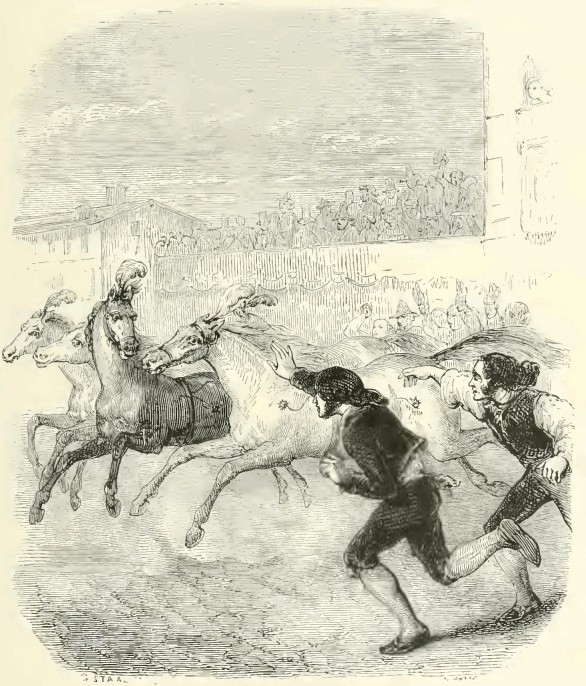
\includegraphics[width=\textwidth]{20199m.jpg}
\end{figure}

“Then it is to your excellency that this letter is addressed.”

“Is there any answer?” inquired Franz, taking the letter from him.

“Yes—your friend at least hopes so.”

“Come upstairs with me, and I will give it to you.”

“I prefer waiting here,” said the messenger, with a smile.

“And why?”

“Your excellency will know when you have read the letter.”

“Shall I find you here, then?”

“Certainly.”

Franz entered the hotel. On the staircase he met Signor Pastrini.
“Well?” said the landlord.

“Well—what?” responded Franz.

“You have seen the man who desired to speak with you from your friend?”
he asked of Franz.

“Yes, I have seen him,” he replied, “and he has handed this letter to
me. Light the candles in my apartment, if you please.”

The innkeeper gave orders to a servant to go before Franz with a light.
The young man had found Signor Pastrini looking very much alarmed, and
this had only made him the more anxious to read Albert’s letter; and so
he went instantly towards the waxlight, and unfolded it. It was written
and signed by Albert. Franz read it twice before he could comprehend
what it contained. It was thus worded:

“My dear Fellow,

“The moment you have received this, have the kindness to take the
letter of credit from my pocket-book, which you will find in the square
drawer of the \textit{secrétaire}; add your own to it, if it be not
sufficient. Run to Torlonia, draw from him instantly four thousand
piastres, and give them to the bearer. It is urgent that I should have
this money without delay. I do not say more, relying on you as you may
rely on me.

“Your friend,

“Albert de Morcerf.

“P.S.—I now believe in Italian \textit{banditti}.”

Below these lines were written, in a strange hand, the following in
Italian:

“\textit{Se alle sei della mattina le quattro mille piastre non sono nelle mie
mani, alla sette il Conte Alberto avrà cessato di vivere}.

“Luigi Vampa.”

“\textit{If by six in the morning the four thousand piastres are not in my
hands, by seven o’clock the Count Albert will have ceased to live}.”

This second signature explained everything to Franz, who now understood
the objection of the messenger to coming up into the apartment; the
street was safer for him. Albert, then, had fallen into the hands of
the famous bandit chief, in whose existence he had for so long a time
refused to believe.

There was no time to lose. He hastened to open the \textit{secrétaire}, and
found the pocket-book in the drawer, and in it the letter of credit.
There were in all six thousand piastres, but of these six thousand
Albert had already expended three thousand.

As to Franz, he had no letter of credit, as he lived at Florence, and
had only come to Rome to pass seven or eight days; he had brought but a
hundred louis, and of these he had not more than fifty left. Thus seven
or eight hundred piastres were wanting to them both to make up the sum
that Albert required. True, he might in such a case rely on the
kindness of Signor Torlonia. He was, therefore, about to return to the
Palazzo Bracciano without loss of time, when suddenly a luminous idea
crossed his mind.

He remembered the Count of Monte Cristo. Franz was about to ring for
Signor Pastrini, when that worthy presented himself.

“My dear sir,” he said, hastily, “do you know if the count is within?”

“Yes, your excellency; he has this moment returned.”

“Is he in bed?”

“I should say no.”

“Then ring at his door, if you please, and request him to be so kind as
to give me an audience.”

Signor Pastrini did as he was desired, and returning five minutes
after, he said:

“The count awaits your excellency.”

Franz went along the corridor, and a servant introduced him to the
count. He was in a small room which Franz had not yet seen, and which
was surrounded with divans. The count came towards him.

“Well, what good wind blows you hither at this hour?” said he; “have
you come to sup with me? It would be very kind of you.”

“No; I have come to speak to you of a very serious matter.”

“A serious matter,” said the count, looking at Franz with the
earnestness usual to him; “and what may it be?”

“Are we alone?”

“Yes,” replied the count, going to the door, and returning. Franz gave
him Albert’s letter.

“Read that,” he said.

The count read it.

“Well, well!” said he.

“Did you see the postscript?”

“I did, indeed.

“\textit{‘Se alle sei della mattina le quattro mille piastre non sono nelle
mie mani, alla sette il conte Alberto avrà cessato di vivere. }

“‘Luigi Vampa.’”

“What think you of that?” inquired Franz.

“Have you the money he demands?”

“Yes, all but eight hundred piastres.”

The count went to his \textit{secrétaire}, opened it, and pulling out a drawer
filled with gold, said to Franz, “I hope you will not offend me by
applying to anyone but myself.”

“You see, on the contrary, I come to you first and instantly,” replied
Franz.

“And I thank you; have what you will;” and he made a sign to Franz to
take what he pleased.

“Is it absolutely necessary, then, to send the money to Luigi Vampa?”
asked the young man, looking fixedly in his turn at the count.

“Judge for yourself,” replied he. “The postscript is explicit.”

“I think that if you would take the trouble of reflecting, you could
find a way of simplifying the negotiation,” said Franz.

“How so?” returned the count, with surprise.

“If we were to go together to Luigi Vampa, I am sure he would not
refuse you Albert’s freedom.”

“What influence can I possibly have over a bandit?”

“Have you not just rendered him a service that can never be forgotten?”

“What is that?”

“Have you not saved Peppino’s life?”

“Well, well,” said the count, “who told you that?”

“No matter; I know it.” The count knit his brows, and remained silent
an instant.

“And if I went to seek Vampa, would you accompany me?”

“If my society would not be disagreeable.”

“Be it so. It is a lovely night, and a walk without Rome will do us
both good.”

“Shall I take any arms?”

“For what purpose?”

“Any money?”

“It is useless. Where is the man who brought the letter?”

“In the street.”

“He awaits the answer?”

“Yes.”

“I must learn where we are going. I will summon him hither.”

“It is useless; he would not come up.”

“To your apartments, perhaps; but he will not make any difficulty at
entering mine.”

The count went to the window of the apartment that looked on to the
street, and whistled in a peculiar manner. The man in the mantle
quitted the wall, and advanced into the middle of the street.
“\textit{Salite!}” said the count, in the same tone in which he would have
given an order to his servant. The messenger obeyed without the least
hesitation, but rather with alacrity, and, mounting the steps at a
bound, entered the hotel; five seconds afterwards he was at the door of
the room.

“Ah, it is you, Peppino,” said the count. But Peppino, instead of
answering, threw himself on his knees, seized the count’s hand, and
covered it with kisses. “Ah,” said the count, “you have, then, not
forgotten that I saved your life; that is strange, for it is a week
ago.”

\begin{figure}[ht]
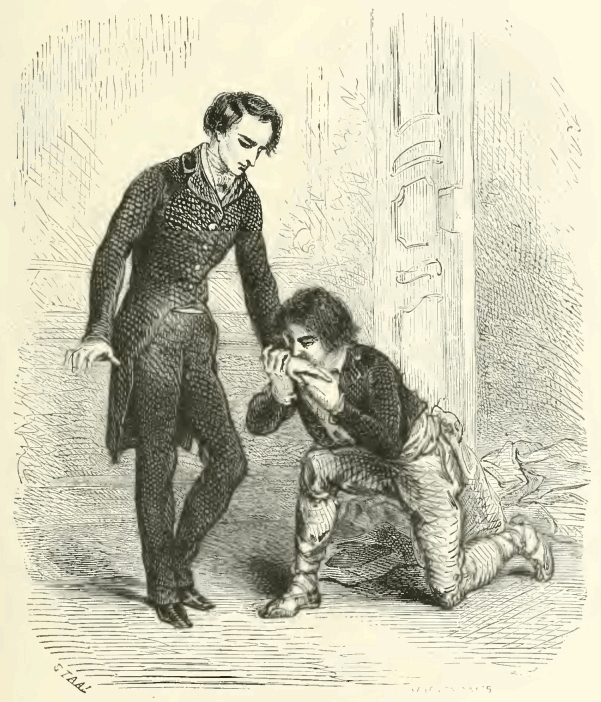
\includegraphics[width=\textwidth]{20203m.jpg}
\end{figure}

“No, excellency; and never shall I forget it,” returned Peppino, with
an accent of profound gratitude.

“Never? That is a long time; but it is something that you believe so.
Rise and answer.”

Peppino glanced anxiously at Franz.

“Oh, you may speak before his excellency,” said he; “he is one of my
friends. You allow me to give you this title?” continued the count in
French, “it is necessary to excite this man’s confidence.”

“You can speak before me,” said Franz; “I am a friend of the count’s.”

“Good!” returned Peppino. “I am ready to answer any questions your
excellency may address to me.”

“How did the Viscount Albert fall into Luigi’s hands?”

“Excellency, the Frenchman’s carriage passed several times the one in
which was Teresa.”

“The chief’s mistress?”

“Yes. The Frenchman threw her a bouquet; Teresa returned it—all this
with the consent of the chief, who was in the carriage.”

“What?” cried Franz, “was Luigi Vampa in the carriage with the Roman
peasants?”

“It was he who drove, disguised as the coachman,” replied Peppino.

“Well?” said the count.

“Well, then, the Frenchman took off his mask; Teresa, with the chief’s
consent, did the same. The Frenchman asked for a rendezvous; Teresa
gave him one—only, instead of Teresa, it was Beppo who was on the steps
of the church of San Giacomo.”

“What!” exclaimed Franz, “the peasant girl who snatched his \textit{mocoletto}
from him——”

“Was a lad of fifteen,” replied Peppino. “But it was no disgrace to
your friend to have been deceived; Beppo has taken in plenty of
others.”

“And Beppo led him outside the walls?” said the count.

“Exactly so; a carriage was waiting at the end of the Via Macello.
Beppo got in, inviting the Frenchman to follow him, and he did not wait
to be asked twice. He gallantly offered the right-hand seat to Beppo,
and sat by him. Beppo told him he was going to take him to a villa a
league from Rome; the Frenchman assured him he would follow him to the
end of the world. The coachman went up the Via di Ripetta and the Porta
San Paolo; and when they were two hundred yards outside, as the
Frenchman became somewhat too forward, Beppo put a brace of pistols to
his head, the coachman pulled up and did the same. At the same time,
four of the band, who were concealed on the banks of the Almo,
surrounded the carriage. The Frenchman made some resistance, and nearly
strangled Beppo; but he could not resist five armed men, and was forced
to yield. They made him get out, walk along the banks of the river, and
then brought him to Teresa and Luigi, who were waiting for him in the
catacombs of St. Sebastian.”

“Well,” said the count, turning towards Franz, “it seems to me that
this is a very likely story. What do you say to it?”

“Why, that I should think it very amusing,” replied Franz, “if it had
happened to anyone but poor Albert.”

“And, in truth, if you had not found me here,” said the count, “it
might have proved a gallant adventure which would have cost your friend
dear; but now, be assured, his alarm will be the only serious
consequence.”

“And shall we go and find him?” inquired Franz.

“Oh, decidedly, sir. He is in a very picturesque place—do you know the
catacombs of St. Sebastian?”

“I was never in them; but I have often resolved to visit them.”

“Well, here is an opportunity made to your hand, and it would be
difficult to contrive a better. Have you a carriage?”

“No.”

“That is of no consequence; I always have one ready, day and night.”

“Always ready?”

“Yes. I am a very capricious being, and I should tell you that
sometimes when I rise, or after my dinner, or in the middle of the
night, I resolve on starting for some particular point, and away I go.”

The count rang, and a footman appeared.

“Order out the carriage,” he said, “and remove the pistols which are in
the holsters. You need not awaken the coachman; Ali will drive.”

In a very short time the noise of wheels was heard, and the carriage
stopped at the door. The count took out his watch.

“Half-past twelve,” he said. “We might start at five o’clock and be in
time, but the delay may cause your friend to pass an uneasy night, and
therefore we had better go with all speed to extricate him from the
hands of the infidels. Are you still resolved to accompany me?”

“More determined than ever.”

“Well, then, come along.”

Franz and the count went downstairs, accompanied by Peppino. At the
door they found the carriage. Ali was on the box, in whom Franz
recognized the dumb slave of the grotto of Monte Cristo. Franz and the
count got into the carriage. Peppino placed himself beside Ali, and
they set off at a rapid pace. Ali had received his instructions, and
went down the Corso, crossed the Campo Vaccino, went up the Strada San
Gregorio, and reached the gates of St. Sebastian. Then the porter
raised some difficulties, but the Count of Monte Cristo produced a
permit from the governor of Rome, allowing him to leave or enter the
city at any hour of the day or night; the portcullis was therefore
raised, the porter had a louis for his trouble, and they went on their
way.

The road which the carriage now traversed was the ancient Appian Way,
and bordered with tombs. From time to time, by the light of the moon,
which began to rise, Franz imagined that he saw something like a
sentinel appear at various points among the ruins, and suddenly retreat
into the darkness on a signal from Peppino.

A short time before they reached the Baths of Caracalla the carriage
stopped, Peppino opened the door, and the count and Franz alighted.

“In ten minutes,” said the count to his companion, “we shall be there.”

He then took Peppino aside, gave him an order in a low voice, and
Peppino went away, taking with him a torch, brought with them in the
carriage. Five minutes elapsed, during which Franz saw the shepherd
going along a narrow path that led over the irregular and broken
surface of the Campagna; and finally he disappeared in the midst of the
tall red herbage, which seemed like the bristling mane of an enormous
lion.

“Now,” said the count, “let us follow him.”

Franz and the count in their turn then advanced along the same path,
which, at the distance of a hundred paces, led them over a declivity to
the bottom of a small valley. They then perceived two men conversing in
the obscurity.

“Ought we to go on?” asked Franz of the count; “or should we pause?”

“Let us go on; Peppino will have warned the sentry of our coming.”

One of the two men was Peppino, and the other a bandit on the lookout.
Franz and the count advanced, and the bandit saluted them.

“Your excellency,” said Peppino, addressing the count, “if you will
follow me, the opening of the catacombs is close at hand.”

“Go on, then,” replied the count. They came to an opening behind a
clump of bushes and in the midst of a pile of rocks, by which a man
could scarcely pass. Peppino glided first into this crevice; after they
got along a few paces the passage widened. Peppino passed, lighted his
torch, and turned to see if they came after him. The count first
reached an open space and Franz followed him closely. The passageway
sloped in a gentle descent, enlarging as they proceeded; still Franz
and the count were compelled to advance in a stooping posture, and were
scarcely able to proceed abreast of one another. They went on a hundred
and fifty paces in this way, and then were stopped by, “Who comes
there?” At the same time they saw the reflection of a torch on a
carbine barrel.

“A friend!” responded Peppino; and, advancing alone towards the sentry,
he said a few words to him in a low tone; and then he, like the first,
saluted the nocturnal visitors, making a sign that they might proceed.

Behind the sentinel was a staircase with twenty steps. Franz and the
count descended these, and found themselves in a mortuary chamber. Five
corridors diverged like the rays of a star, and the walls, dug into
niches, which were arranged one above the other in the shape of
coffins, showed that they were at last in the catacombs. Down one of
the corridors, whose extent it was impossible to determine, rays of
light were visible. The count laid his hand on Franz’s shoulder.

“Would you like to see a camp of bandits in repose?” he inquired.

“Exceedingly,” replied Franz.

“Come with me, then. Peppino, put out the torch.” Peppino obeyed, and
Franz and the count were in utter darkness, except that fifty paces in
advance of them a reddish glare, more evident since Peppino had put out
his torch, was visible along the wall.

They advanced silently, the count guiding Franz as if he had the
singular faculty of seeing in the dark. Franz himself, however, saw his
way more plainly in proportion as he went on towards the light, which
served in some manner as a guide. Three arcades were before them, and
the middle one was used as a door. These arcades opened on one side
into the corridor where the count and Franz were, and on the other into
a large square chamber, entirely surrounded by niches similar to those
of which we have spoken.

In the midst of this chamber were four stones, which had formerly
served as an altar, as was evident from the cross which still
surmounted them. A lamp, placed at the base of a pillar, lighted up
with its pale and flickering flame the singular scene which presented
itself to the eyes of the two visitors concealed in the shadow.

A man was seated with his elbow leaning on the column, and was reading
with his back turned to the arcades, through the openings of which the
new-comers contemplated him. This was the chief of the band, Luigi
Vampa. Around him, and in groups, according to their fancy, lying in
their mantles, or with their backs against a sort of stone bench, which
went all round the columbarium, were to be seen twenty brigands or
more, each having his carbine within reach. At the other end, silent,
scarcely visible, and like a shadow, was a sentinel, who was walking up
and down before a grotto, which was only distinguishable because in
that spot the darkness seemed more dense than elsewhere.

When the count thought Franz had gazed sufficiently on this picturesque
tableau, he raised his finger to his lips, to warn him to be silent,
and, ascending the three steps which led to the corridor of the
columbarium, entered the chamber by the middle arcade, and advanced
towards Vampa, who was so intent on the book before him that he did not
hear the noise of his footsteps.

“Who comes there?” cried the sentinel, who was less abstracted, and who
saw by the lamp-light a shadow approaching his chief. At this
challenge, Vampa rose quickly, drawing at the same moment a pistol from
his girdle. In a moment all the bandits were on their feet, and twenty
carbines were levelled at the count.

“Well,” said he in a voice perfectly calm, and no muscle of his
countenance disturbed, “well, my dear Vampa, it appears to me that you
receive a friend with a great deal of ceremony.”

\begin{figure}[h]
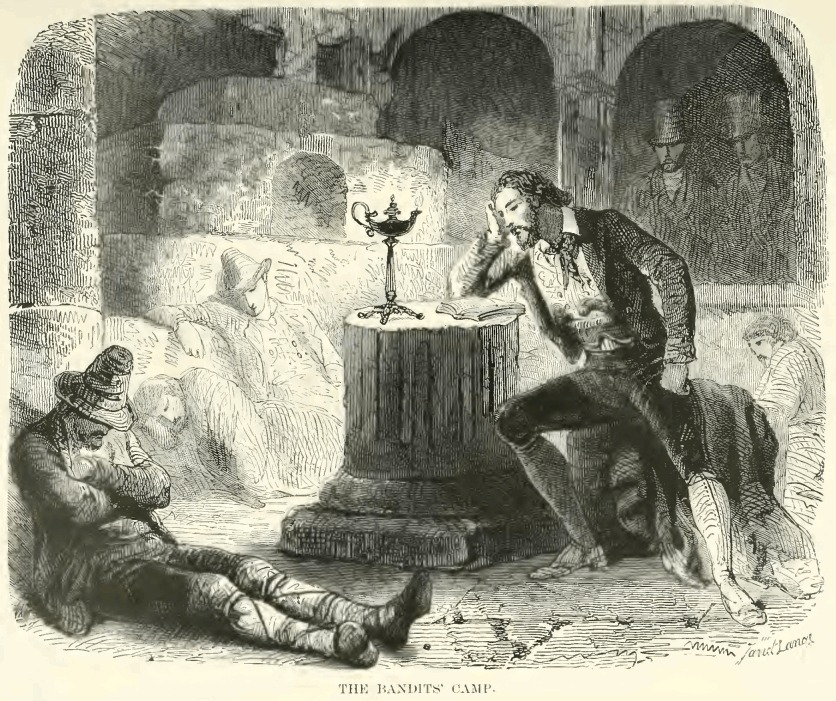
\includegraphics[width=\textwidth]{20207m.jpg}
\end{figure}

“Ground arms,” exclaimed the chief, with an imperative sign of the
hand, while with the other he took off his hat respectfully; then,
turning to the singular personage who had caused this scene, he said,
“Your pardon, your excellency, but I was so far from expecting the
honor of a visit, that I did not really recognize you.”

“It seems that your memory is equally short in everything, Vampa,” said
the count, “and that not only do you forget people’s faces, but also
the conditions you make with them.”

“What conditions have I forgotten, your excellency?” inquired the
bandit, with the air of a man who, having committed an error, is
anxious to repair it.

“Was it not agreed,” asked the count, “that not only my person, but
also that of my friends, should be respected by you?”

“And how have I broken that treaty, your excellency?”

“You have this evening carried off and conveyed hither the Viscount
Albert de Morcerf. Well,” continued the count, in a tone that made
Franz shudder, “this young gentleman is one of \textit{my friends}—this young
gentleman lodges in the same hotel as myself—this young gentleman has
been up and down the Corso for eight hours in my private carriage, and
yet, I repeat to you, you have carried him off, and conveyed him
hither, and,” added the count, taking the letter from his pocket, “you
have set a ransom on him, as if he were an utter stranger.”

“Why did you not tell me all this—you?” inquired the brigand chief,
turning towards his men, who all retreated before his look. “Why have
you caused me thus to fail in my word towards a gentleman like the
count, who has all our lives in his hands? By heavens! if I thought one
of you knew that the young gentleman was the friend of his excellency,
I would blow his brains out with my own hand!”

\begin{figure}[ht]
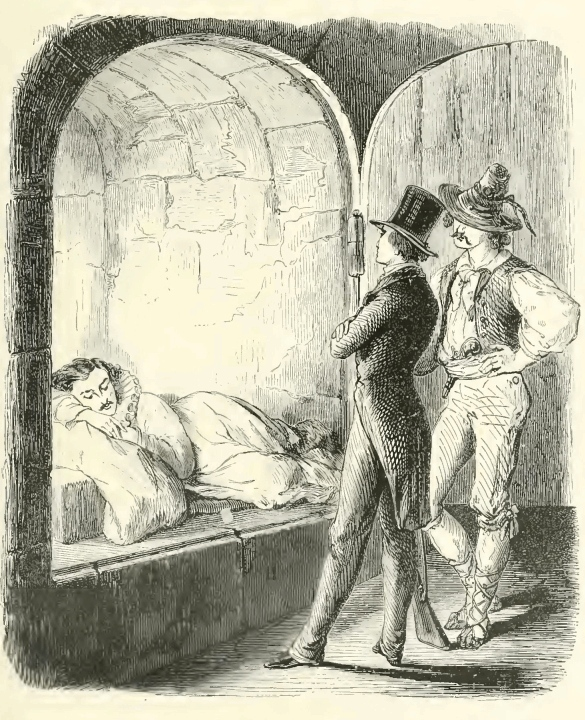
\includegraphics[width=\textwidth]{20211m.jpg}
\end{figure}

“Well,” said the count, turning towards Franz, “I told you there was
some mistake in this.”

“Are you not alone?” asked Vampa with uneasiness.

“I am with the person to whom this letter was addressed, and to whom I
desired to prove that Luigi Vampa was a man of his word. Come, your
excellency,” the count added, turning to Franz, “here is Luigi Vampa,
who will himself express to you his deep regret at the mistake he has
committed.”

Franz approached, the chief advancing several steps to meet him.

“Welcome among us, your excellency,” he said to him; “you heard what
the count just said, and also my reply; let me add that I would not for
the four thousand piastres at which I had fixed your friend’s ransom,
that this had happened.”

“But,” said Franz, looking round him uneasily, “where is the
viscount?—I do not see him.”

“Nothing has happened to him, I hope,” said the count frowningly.

“The prisoner is there,” replied Vampa, pointing to the hollow space in
front of which the bandit was on guard, “and I will go myself and tell
him he is free.”

The chief went towards the place he had pointed out as Albert’s prison,
and Franz and the count followed him.

“What is the prisoner doing?” inquired Vampa of the sentinel.

“\textit{Ma foi}, captain,” replied the sentry, “I do not know; for the last
hour I have not heard him stir.”

“Come in, your excellency,” said Vampa. The count and Franz ascended
seven or eight steps after the chief, who drew back a bolt and opened a
door. Then, by the gleam of a lamp, similar to that which lighted the
columbarium, Albert was to be seen wrapped up in a cloak which one of
the bandits had lent him, lying in a corner in profound slumber.

“Come,” said the count, smiling with his own peculiar smile, “not so
bad for a man who is to be shot at seven o’clock tomorrow morning.”

Vampa looked at Albert with a kind of admiration; he was not insensible
to such a proof of courage.

“You are right, your excellency,” he said; “this must be one of your
friends.”

Then going to Albert, he touched him on the shoulder, saying, “Will
your excellency please to awaken?”

Albert stretched out his arms, rubbed his eyelids, and opened his eyes.

“Oh,” said he, “is it you, captain? You should have allowed me to
sleep. I had such a delightful dream. I was dancing the galop at
Torlonia’s with the Countess G——.” Then he drew his watch from his
pocket, that he might see how time sped.

“Half-past one only?” said he. “Why the devil do you rouse me at this
hour?”

“To tell you that you are free, your excellency.”

“My dear fellow,” replied Albert, with perfect ease of mind, “remember,
for the future, Napoleon’s maxim, ‘Never awaken me but for bad news;’
if you had let me sleep on, I should have finished my galop, and have
been grateful to you all my life. So, then, they have paid my ransom?”

“No, your excellency.”

“Well, then, how am I free?”

“A person to whom I can refuse nothing has come to demand you.”

“Come hither?”

“Yes, hither.”

“Really? Then that person is a most amiable person.”

Albert looked around and perceived Franz. “What,” said he, “is it you,
my dear Franz, whose devotion and friendship are thus displayed?”

“No, not I,” replied Franz, “but our neighbor, the Count of Monte
Cristo.”

“Oh, my dear count,” said Albert gayly, arranging his cravat and
wristbands, “you are really most kind, and I hope you will consider me
as under eternal obligations to you, in the first place for the
carriage, and in the next for this visit,” and he put out his hand to
the count, who shuddered as he gave his own, but who nevertheless did
give it.

The bandit gazed on this scene with amazement; he was evidently
accustomed to see his prisoners tremble before him, and yet here was
one whose gay temperament was not for a moment altered; as for Franz,
he was enchanted at the way in which Albert had sustained the national
honor in the presence of the bandit.

“My dear Albert,” he said, “if you will make haste, we shall yet have
time to finish the night at Torlonia’s. You may conclude your
interrupted galop, so that you will owe no ill-will to Signor Luigi,
who has, indeed, throughout this whole affair acted like a gentleman.”

“You are decidedly right, and we may reach the Palazzo by two o’clock.
Signor Luigi,” continued Albert, “is there any formality to fulfil
before I take leave of your excellency?”

“None, sir,” replied the bandit, “you are as free as air.”

“Well, then, a happy and merry life to you. Come, gentlemen, come.”

And Albert, followed by Franz and the count, descended the staircase,
crossed the square chamber, where stood all the bandits, hat in hand.

“Peppino,” said the brigand chief, “give me the torch.”

“What are you going to do?” inquired the count.

“I will show you the way back myself,” said the captain; “that is the
least honor that I can render to your excellency.”

And taking the lighted torch from the hands of the herdsman, he
preceded his guests, not as a servant who performs an act of civility,
but like a king who precedes ambassadors. On reaching the door, he
bowed.

“And now, your excellency,” added he, “allow me to repeat my apologies,
and I hope you will not entertain any resentment at what has occurred.”

“No, my dear Vampa,” replied the count; “besides, you compensate for
your mistakes in so gentlemanly a way, that one almost feels obliged to
you for having committed them.”

\begin{figure}[ht]
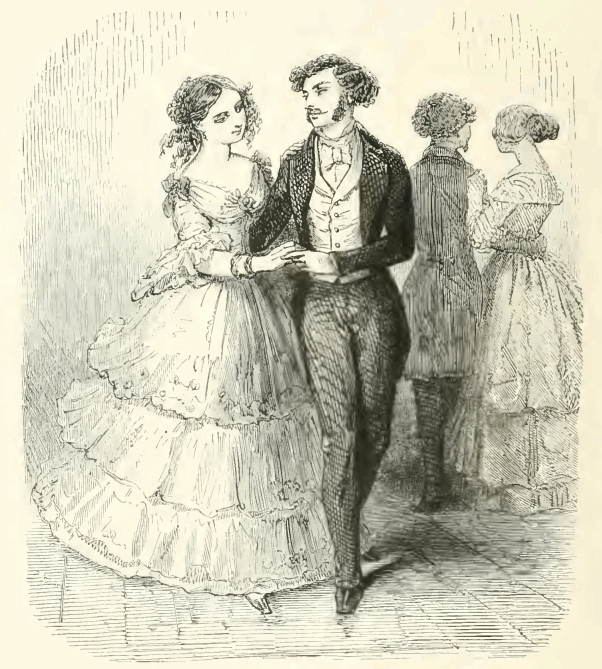
\includegraphics[width=\textwidth]{20214m.jpg}
\end{figure}

“Gentlemen,” added the chief, turning towards the young men, “perhaps
the offer may not appear very tempting to you; but if you should ever
feel inclined to pay me a second visit, wherever I may be, you shall be
welcome.”

Franz and Albert bowed. The count went out first, then Albert. Franz
paused for a moment.

“Has your excellency anything to ask me?” said Vampa with a smile.

“Yes, I have,” replied Franz; “I am curious to know what work you were
perusing with so much attention as we entered.”

“Cæsar’s \textit{Commentaries},” said the bandit, “it is my favorite work.”

“Well, are you coming?” asked Albert.

“Yes,” replied Franz, “here I am,” and he, in his turn, left the caves.
They advanced to the plain.

“Ah, your pardon,” said Albert, turning round; “will you allow me,
captain?”

And he lighted his cigar at Vampa’s torch.

“Now, my dear count,” he said, “let us on with all the speed we may. I
am enormously anxious to finish my night at the Duke of Bracciano’s.”

They found the carriage where they had left it. The count said a word
in Arabic to Ali, and the horses went on at great speed.

It was just two o’clock by Albert’s watch when the two friends entered
into the dancing-room. Their return was quite an event, but as they
entered together, all uneasiness on Albert’s account ceased instantly.

“Madame,” said the Viscount of Morcerf, advancing towards the countess,
“yesterday you were so condescending as to promise me a galop; I am
rather late in claiming this gracious promise, but here is my friend,
whose character for veracity you well know, and he will assure you the
delay arose from no fault of mine.”

And as at this moment the orchestra gave the signal for the waltz,
Albert put his arm round the waist of the countess, and disappeared
with her in the whirl of dancers.

In the meanwhile Franz was considering the singular shudder that had
passed over the Count of Monte Cristo at the moment when he had been,
in some sort, forced to give his hand to Albert.
